% !TEX root = ../main.tex

\chapter{Technical development} % (fold)
\label{chp:execution}

\section{Terminology}
\label{sec:terminology}

The Algolia API is pushing by uploading schemaless JSON objects to an index

\section{Organizing state} % (fold)
\label{sec:organizing_state}

\subsection{Widgets and connectors}
\label{sub:widgets_and_connectors}

The big difference between using Algolia with the Helper compared to InstantSearch is the notion of widgets. In the current implementations there are ten core widgets. Each of these widgets is split up in its logic (a connector) and its display logic (a component). Together these widgets are:

\begin{itemize}
  \item SearchBox
  \item Hits
  \item RefinementList
  \item Range
  \item Pagination
  \item ClearAll
  \item CurrentRefinements
  \item Sort By
  \item Highlight
  \item Snippet
\end{itemize}

There are two kinds of widgets, interactive widgets and display-only widgets. Display-only widgets read the current results and applied refinements from the Algolia response. The display-only widgets are Hits, which is a representation of all the results. The other two are Highlight and Snippet, which take an attributen, and display the snipped and highlighted result from the Algolia response.

The other widgets are interactive widgets. They also take their display value from the response, to show which facets are enabled, or which refinement is already made. All of them also expose a {\tt refine()} function. This function will be called whenever is applicable in that case, and uses Helper methods like {\tt helper.state.toggleRefinement} to actually apply their change on the search state.

%%
talk about the difference between storing parameters and storing widget state

\subsection{Structuring a state container}
\label{sub:structuring_a_state_container}

In the InstantSearch Core implementation the choice has been made to structure state in three divisions. One for the result that comes from each API call, one for raw parameters like {\tt DISTINCT} and another division for the actual refinements.

... % 

Finally the state looks like this


\begin{lstlisting}[caption={Using instantsearch-core},label={lst:is-core-usage}]
const state = {
  refinements: {
    color: {
      type: 'menu',
      value: 'blue',
    },
    brand: {
      type: 'list',
      value: ['apple', 'samsung'],
    },
    price: {
      type: 'range',
      value: '>= 5',
    },
    query: {
      type: 'query',
      value: '',
    },
  },
  rawParameters: {
    distinct: true,
    page: 3,
  },
  result: {
    processingTimeMS: 5,
    filters: {
      color: [
        { label: 'red', value: 10 },
        { label: 'blue', value: 100 },
        { label: 'orange', value: 1 },
      ],
    },
    hits: [
      {
        objectID: '0x1f355',
        color: 'blue',
      },
    ],
  },
};
\end{lstlisting}

connectors are easier when you can just have one listener / changer per connector type. Don't care about the global state basically.

% section organizing_state (end)

\section{Handling state changes} % (fold)
\label{sec:handling_state_changes}

%%
Research:

\begin{itemize}
  \item observables vs flux
  \item Other languages (Elm model)\cite{csstricks-elm}
\end{itemize}

% section handling_state_changes (end)

\section{Getting responses from the API} % (fold)
\label{sec:getting_responses_from_the_api}

another function listens to changes in state

it transforms params into a JS client request

it replaces the {\tt response} in the state with an action

% section getting_responses_from_the_api (end)

\section{Rendering refinements} % (fold)
\label{sec:rendering_refinements}

Stuff to think about: dynamic facets as core part of this API or not?

% section rendering_refinements (end)

\section{Saved state} % (fold)
\label{sec:saved_state}

allow for replacing of whole state

reasons

\begin{enumerate}
  \item saving state in url
  \item saving state in localstorage
  \item SSR
\end{enumerate}

documentation very clear that this shouldn't regularly be used

% section saved_state (end)

\section{Overview} % (fold)
\label{sec:overview}

\begin{figure}[H]
\label{figure:core-architecture}
  \centering
  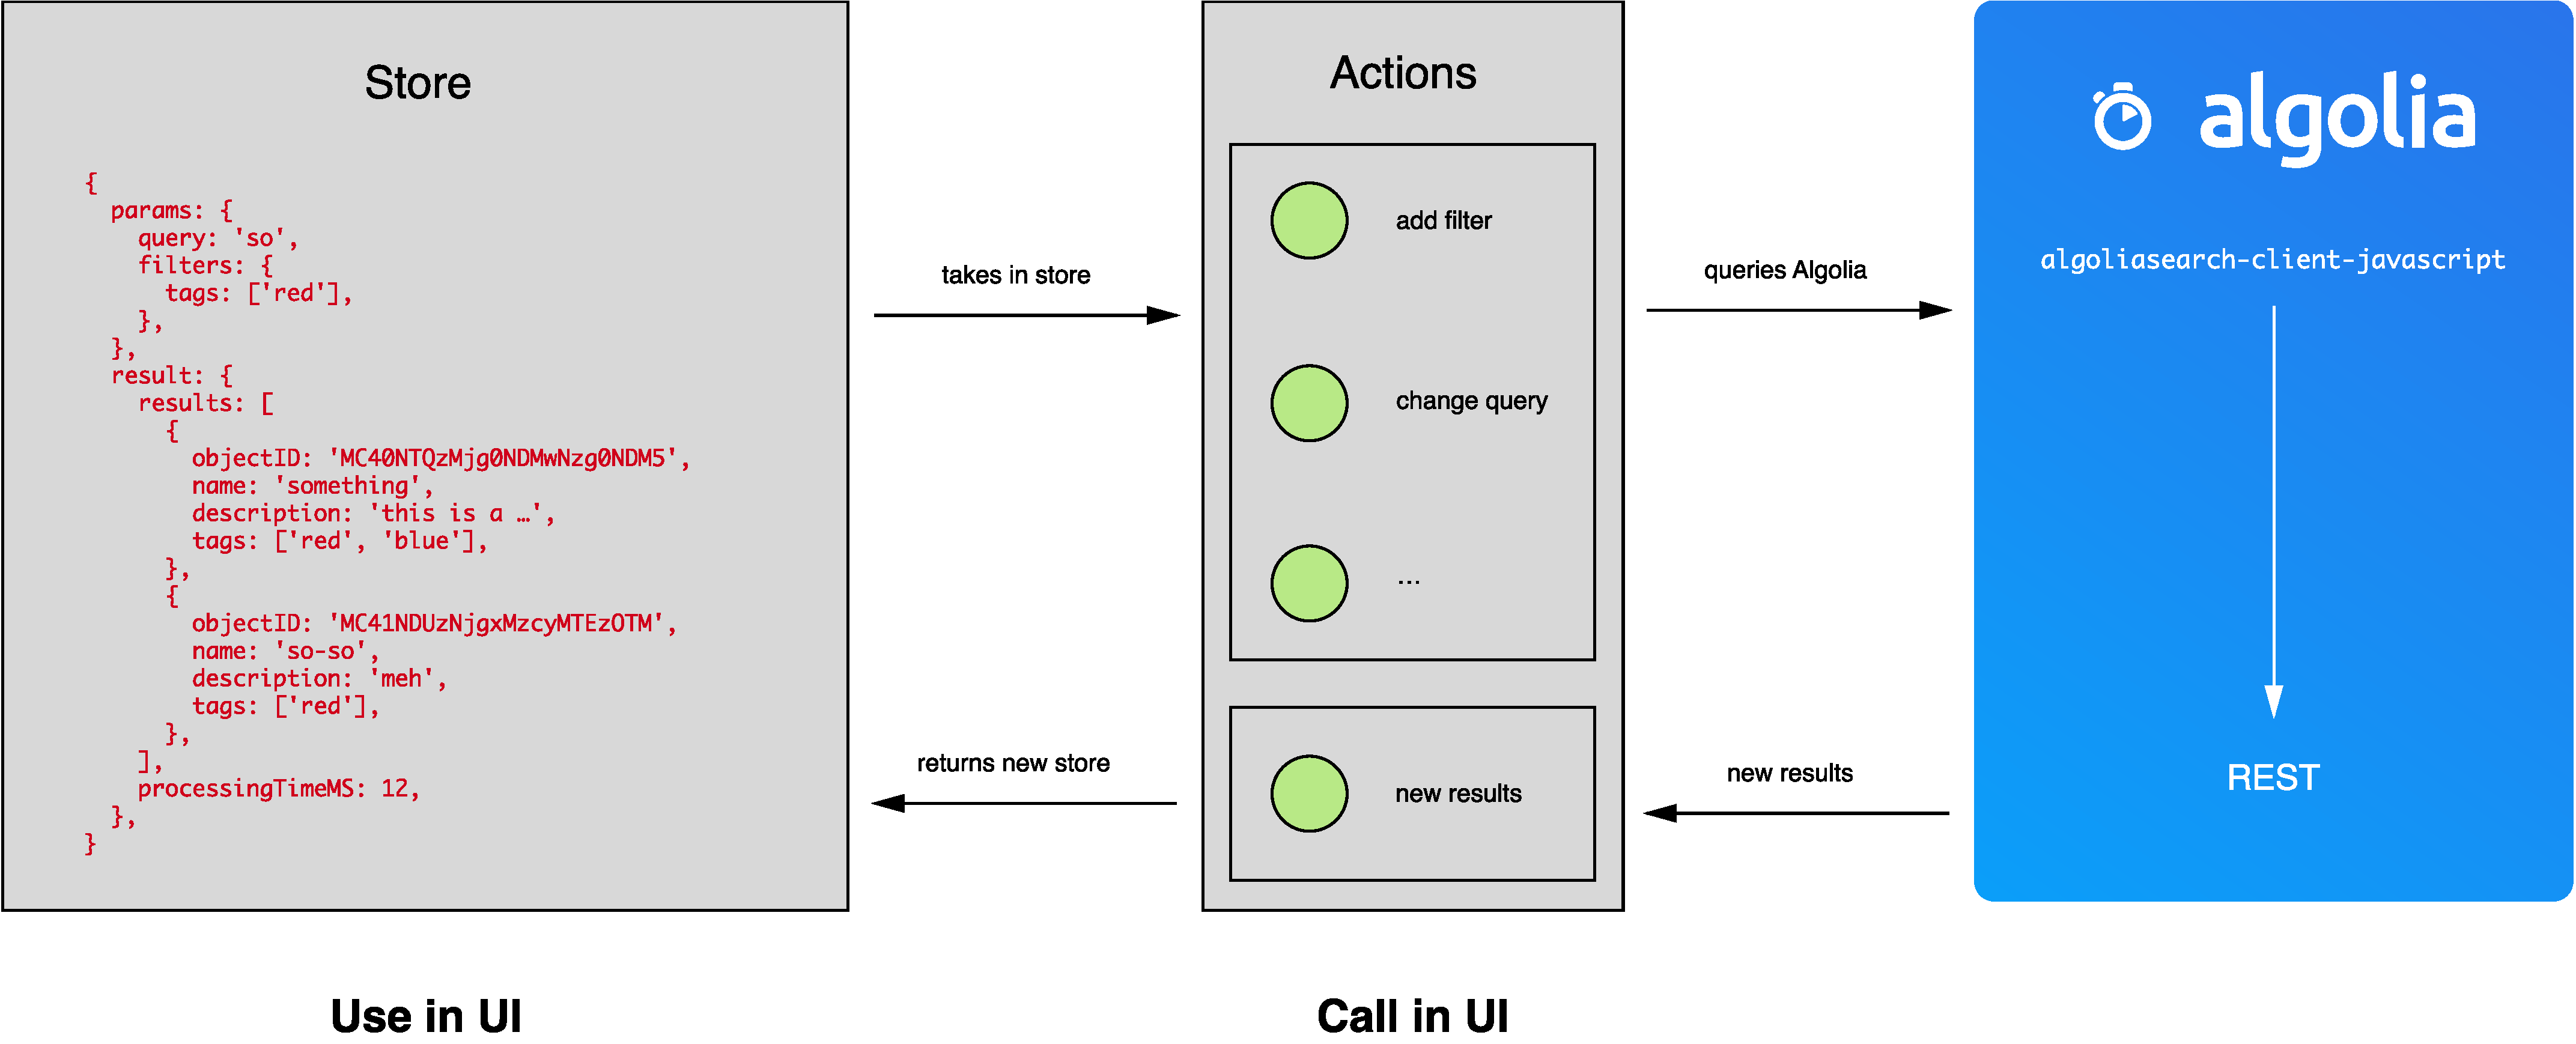
\includegraphics[width=\textwidth]{../assets/architecture.pdf}
  \caption{Architecture overview\cite{blog-architecture}}
\end{figure}

% section overview (end)

\section{Usage in libraries} % (fold)
\label{sec:usage_in_libraries}

PoC in instantsearch.js and ReactInstantsearch for the RefinementList %%

% section usage_in_libraries (end)

\section{Complete implementation} % (fold)
\label{sec:complete_implementation}

Obviously this isn't final and too detailed.

\begin{lstlisting}[caption={Using instantsearch-core},label={lst:is-core-usage}]
// stores.js
import algoliasearch from 'algoliasearch';
import { createStore } from 'instantsearch-core';

const appId = 'OFCNCOG2CU';
const apiKey = 'f54e21fa3a2a0160595bb058179bfb1e';
const indexName = 'products_asc';

const client = algoliasearch(appId, apiKey);
const productsStore = createStore(client, indexName);

export productsStore;

// widget.js
import { setQuery } from 'instantsearch-core/actions/query';
import { productsStore } from './stores';

function onInput(event) {
  event.preventDefault();

  productsStore.refine(setQuery(event.target.value));
}
\end{lstlisting}

% section complete_implementation (end)

